\documentclass[10pt, titlepage]{article}

\usepackage[margin=1in]{geometry}
\usepackage{fancyhdr}
\usepackage{amsfonts}
\usepackage{amsmath}
\usepackage{amssymb}
\usepackage{booktabs}
\usepackage{tikz}
\usepackage{pgfplots}
\usepackage{float}
\usepackage{bm}


\title{\normalsize PLUS Session Worksheet \\[1em] \Large \textit{MATH 1554:} Linear Algebra}
\author{Covering lessons: 5.3 \& 5.5}
\date{Fall 2023}

% ------- Set up header -------
\renewcommand{\sectionmark}[1]{\markright{#1}} % from https://tex.stackexchange.com/a/317393/227665
\pagestyle{fancy}
\fancyhead[L]{Fall 2023}
%\fancyhead[C]{\textit{\nouppercase{\rightmark}}}
\fancyhead[C]{\textit{Diagonalization (5.3) \& Complex Eigenvalues (5.5)}}
\fancyhead[R]{\textbf{\thepage}}
% -------------------------------------------------------

% ------- Set up Main Idea box environment -------
\newcounter{mainideas}
\setcounter{mainideas}{1}
\newcommand{\mainidea}{\textbf{Main Idea \#\themainideas \stepcounter{mainideas}}}
\setlength\fboxsep{1em}
%\newcommand{\midea}[2]{\begin{center}\fbox{\parbox{#1}{\centering \mainidea #2}} \end{center}} % Could be environment but I couldn't bother

% The way this works is that the savebox collects whatever was between the minipage and the end of it, then in the last line of the definition of the environment
% we regurgigate whatever was collected into an fbox which we center.
\newsavebox{\mybox}
\newenvironment{mideea}[1]
{%
\begin{lrbox}{\mybox}%
	\begin{minipage}{#1\textwidth}
		{\centering \mainidea \par}

}
{\end{minipage}\end{lrbox}\begin{center}\fbox{\usebox{\mybox}}\end{center}}
% -------------------------------------------------------

% ------- Set up activity environment -------
\newcounter{question}
\setcounter{question}{1}
\newenvironment{newquestion}
{
	\noindent\textbf{Question \thequestion}
}
{
\stepcounter{question}
\par
}
% -------------------------------------------------------


% ------- Set up math stuff -------
\renewcommand{\vec}[1]{\bm{#1}}
\DeclareMathOperator{\vspan}{Span}
\DeclareMathOperator{\row}{row}
\DeclareMathOperator{\col}{col}
\DeclareMathOperator{\colspace}{Col}
\DeclareMathOperator{\nullspace}{Nul}
\DeclareMathOperator{\rank}{rank}
% -------------------------------------------------------

% ------- Set up circle -------
\newcommand{\bubble}{\tikz[baseline=-0.625ex]\draw[radius=0.5em, fill=white] (0,0) circle;}
\newcommand{\dbubble}{\tikz[baseline=-0.625ex]\draw[radius=0.5em, fill=black] (0,0) circle;}
% -------------------------------------------------------

\begin{document}
\maketitle

\section{\centering Diagonalization (5.3)}
	\begin{mideea}{0.9}
		If the eigenvectors of a matrix \(A \in \mathbb{R}^{n \times n}\) form a basis for \(\mathbb{R}^n\), then it is possible to write \(A\) in the form of 
		\[A = PDP^{-1},\] where the columns of \(P\) are the eigenvectors of \(A\) and the entries of the diagonal matrix \(D\) are the corresponding 
		eigenvalues.
	\end{mideea}

	\begin{newquestion}
		For the following statements, answer \textit{true} if the statement is always true, and \textit{false} otherwise.
		\begin{table}[!h]
			\centering
			\begin{tabular}{c@{\hspace{2.5em}}cp{0.75\textwidth}}
				true & false & \\
				\specialrule{\lightrulewidth}{0.25em}{1.25em}
				\bubble & \bubble & It is possible that there exists a square matrix \(A\) that is similar to a diagonalizable matrix \(B\), but \(A\) isn't diagonalizable. \\[0.75em]
				\bubble & \bubble & If \(\vec{x}\) is an eigenvector of \(A\) with corresponding eigenvalue of \(\lambda\), and \(A = PBP^{-1}\) for some
							      matrix \(P\), then \(P^{-1}\vec{x}\) is an eigenvector of \(B\) with corresponding eigenvalue \(\lambda\). \\[0.75em]
				\bubble & \bubble & Row-equivalent matrices are similar. \\[0.75em]
				\bubble & \bubble & Two similar matrices have the same eigenvalues.*\\[0.75em]
				\bottomrule
			\end{tabular}
		\end{table}
	\end{newquestion}

	\begin{newquestion}
		Refer to \textit{Sample Final Exam A}, Q. 12.
	\end{newquestion}

\section{\centering Complex Eigenvalues (5.5)}
	\begin{mideea}{0.9}
		It is possibe for a real matrix to have complex eigenvalues and eigenvectors. If that is the case, the eigen-stuff come in \emph{conjugate pairs}. That is, if \(\lambda\) is a
		complex eigenvalue of \(A\) with a corresponding complex eigenvector \(\vec{v}\), then \(\overline{\lambda}\) is an eigenvalue of \(A\) and \(\overline{\vec{v}}\) is the 
		corresponding eigenvector.\footnote{\(\overline{\lambda}\) denotes the complex conjugate of \(\lambda\).}
	\end{mideea}

	\begin{newquestion}
		Answer the following statements with \textit{possible} if the statement \emph{could} be true, or \textit{impossible} otherwise.
		\begin{table}[!h]
			\centering
			\begin{tabular}{c@{\hspace{2.5em}}cp{0.75\textwidth}}
				possible & impossible & \\
				\specialrule{\lightrulewidth}{0.25em}{1.25em}
				\bubble & \bubble & A real \(5 \times 5\) matrix that has 3 complex eigenvalues and 2 real eigenvalues. \\[0.75em]
				\bubble & \bubble & A real \(2 \times 2\) matrix that has \(1 + 5i\) and \(-1 + 5i\) as eigenvalues. \\[0.75em]
				\bubble & \bubble & A real \(3 \times 3\) matrix that has a real eigenvalue and 2 complex eigenvalues. \\[0.75em]
				\bubble & \bubble & A real \(n \times n\) matrix where \(n\) is odd and none of the eigenvalues of the matrix are real. \\[0.75em]
				\bottomrule
			\end{tabular}
		\end{table}
	\end{newquestion}

	\begin{newquestion}
		\(A = \begin{pmatrix}2 & -1 \\ 1 & 2\end{pmatrix}\) has an eigenvalue of \(\lambda_1 = 2 + i\). Find \(\lambda_2\) and the corresponding 
		eigenvectors \(\vec{v}_1\) (corresponds to \(\lambda_1\)) and \(\vec{v}_2\) (corresponds to \(\lambda_2\)).
	\end{newquestion}


\fancyhead[C]{\textit{Solutions}}

\section{Solutions}

\subsection{Solutions to \textit{Diagonalization} Section}

\subsubsection{Solutions to T/F Questions}
	\begin{table}[!h]
		\centering
		\begin{tabular}{c@{\hspace{2.5em}}cp{0.75\textwidth}}
			true & false & \\
			\specialrule{\lightrulewidth}{0.25em}{1.25em}
			\bubble & \dbubble & It is possible that there exists a square matrix \(A\) that is similar to a diagonalizable matrix \(B\), but \(A\) isn't diagonalizable. \\[0.75em]
			\dbubble & \bubble & If \(\vec{x}\) is an eigenvector of \(A\) with corresponding eigenvalue of \(\lambda\), and \(A = PBP^{-1}\) for some
						      matrix \(P\), then \(P^{-1}\vec{x}\) is an eigenvector of \(B\) with corresponding eigenvalue \(\lambda\). \\[0.75em]
			\bubble & \dbubble & Row-equivalent matrices are similar. \\[0.75em]
			\dbubble & \bubble & Two similar matrices have the same eigenvalues.*\\[0.75em]
			\bottomrule
		\end{tabular}
	\end{table}

\subsubsection{Solutions to \textit{Q2}}
	For (i), \(\lambda_1 = 1/2\), \(\lambda_2=2\). For (ii), look at sketch below.
	\begin{figure}[!h]
		\centering
		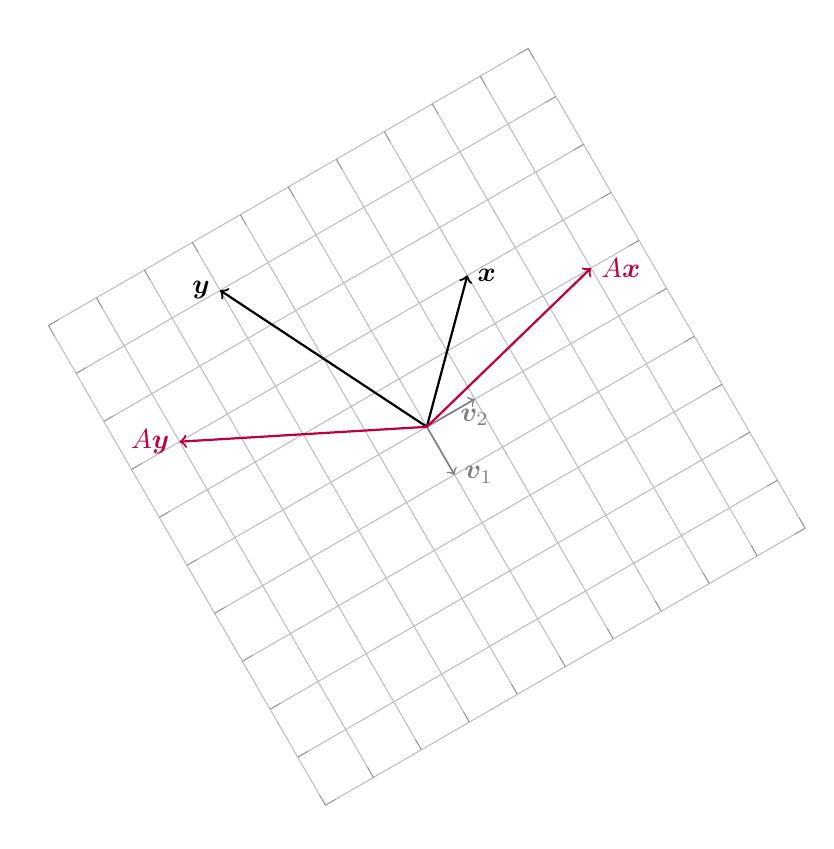
\begin{tikzpicture}
			\begin{axis}[scale=20, grid=major, axis line style={draw=none}, xmin=-5,xmax=5,ymin=-5,ymax=5, xtick distance=1,
					   ytick distance=1,y={({sqrt(3)*0.5}, 0.5)}, x={(0.5, {-sqrt(3)*0.5})}, xticklabel=\empty, yticklabel=\empty]
				\addplot[semithick, ->, gray] coordinates {(0, 0) (0, 1)} node[below] {\(\vec{v}_2\)};
				\addplot[semithick, ->, gray] coordinates {(0, 0) (1, 0)} node[right] {\(\vec{v}_1\)};
	
				\addplot[thick, ->] coordinates {(0, 0) (-2, 2)} node[right] {\(\vec{x}\)};
				\addplot[thick, ->] coordinates {(0, 0) (-4, -2)} node[left] {\(\vec{y}\)};
	
				\addplot[thick, ->, purple] coordinates {(0, 0) (-2, -4)} node[left] {\(A\vec{y}\)};
				\addplot[thick, ->, purple] coordinates {(0, 0) (-1, 4)} node[right] {\(A\vec{x}\)};
			\end{axis}
		\end{tikzpicture}
	\end{figure}

	For (iii), consider that any vector \(\vec{w} \in \mathbb{R}^2\) could be written as a linear combination of \(\vec{v}_1, \vec{v}_2\). That is, any vector 
	\(\vec{w}\) could be expressed as follows \[\vec{w} = c_1\vec{v}_1 + c_2\vec{v}_2.\] Applying \(A\) to \(\vec{w}\) amounts to scaling the weights
	(coordinates!) \(c_1, c_2\). That is, \[A\vec{w} = Ac_1\vec{v}_1 + Ac_2\vec{v}_2 = \lambda_1c_1\vec{v}_1 + \lambda_2c_2\vec{v}_2.\]
	Thus, applying \(A\) \(k\) times could be expressed as \[A^k\vec{w} = \lambda_1^kc_1\vec{v}_1 + \lambda_2^kc_2\vec{v}_2.\]
	
	Since \(\lvert\lambda_2\rvert > 1\), which means that \(\lambda_2^kc \to \infty\) as \(k \to \infty\). To avoid this, our vector \(\vec{w}\) must not have
	any component reliant on \(\vec{v}_2\). (\(c_2 = 0\).) So any vector \(\vec{w} = c_1\vec{v}_1\) with \(c_1 \in \mathbb{R}\) works.

\subsection{Solutions to \textit{Complex Eigenvalues} Section}
	\subsubsection{Solutions to Possible/Impossible Questions}
	\begin{table}[!h]
		\centering
		\begin{tabular}{c@{\hspace{2.5em}}cp{0.75\textwidth}}
			possible & impossible & \\
			\specialrule{\lightrulewidth}{0.25em}{1.25em}
			\bubble & \dbubble & A real \(5 \times 5\) matrix that has 3 complex eigenvalues and 2 real eigenvalues. \\[0.75em]
			\bubble & \dbubble & A real \(2 \times 2\) matrix that has \(1 + 5i\) and \(-1 + 5i\) as eigenvalues. \\[0.75em]
			\dbubble & \bubble & A real \(3 \times 3\) matrix that has a real eigenvalue and 2 complex eigenvalues. \\[0.75em]
			\bubble & \dbubble & A real \(n \times n\) matrix where \(n\) is odd and none of the eigenvalues of the matrix are real. \\[0.75em]
			\bottomrule
		\end{tabular}
	\end{table}

\subsubsection{Solutions to \textit{Q4}}
	We automatically know that the second eigenvalue is \(2 - i\). We now have to find a basis for each eigenspace. We use the usual method. For 
	\(\lambda_1 = 2 + i\):
	\[\begin{pmatrix}2 - (2 + i) & -1 \\ 1 & 2 - (2 + i)\end{pmatrix} = \begin{pmatrix}-i & -1 \\ 1 & -i\end{pmatrix} \sim \begin{pmatrix} 1 & -i \\ 0 & 0\end{pmatrix}.\] 

	So the paramteric vector form of the solution set is \(\vec{x} = t\begin{pmatrix}i \\ 1\end{pmatrix}\). Choose 
	\(\vec{v} = \begin{pmatrix}i \\ 1\end{pmatrix}\).

	We know that the conjugate of a complex eigenvector is also an eigenvector of a real matrix, so the corresponding paramteric vector form for the 
	solution set is \(\vec{y} = t\begin{pmatrix}-i \\ 1\end{pmatrix}\). Choose \(\vec{v}_2 = \begin{pmatrix}-i \\ 1\end{pmatrix}\). 
	
\end{document}
